
\subsection{Performance Formula}
\label{sub-sec:formula}
Although in the IT industry the performance of the applications can be measured by a variety of metrics like: number of concurrent users, up-time and response time, the performance of a person can only be determined only by the way that the employee objectives have been fulfilled. 
But in order for an employee to follow his objectives, both he and his manager have to be aware that performance is a mix of knowledge, willingness and setting.
\begin{equation}
\label{math:perf}
PERFOMANCE = WANT \times CAN \times HAS\ THE\ NECESSARY\ SETTING
\end{equation}

Although the performance varies over time, usually it is favoured by the three keys in \cref{math:perf}. The terms can be interpreted as:
\begin{description}
\item[Want] The person executing the task desires to work on it, finding it interesting enough and being worth it's time.
\item[Can] The person working on the task has enough knowledge to finish the task, without having to spend more de half of the time necessary for it just to gain the necessary knowledge. 
\item[Has the setting] All the necessary requirements (eg: hardware, trainings, basic necessities) are provided prior to developing the task.
\end{description}

For the third item, in general the manager is accountable for, it is his responsibility to provide the necessary environment so that his employees can do their job in a good and stable manner. For example, if a new project is started in Scala with people who have experience on Java and are willing to learn new languages, he must be the one to provide trainings (online, paid, etc.) so that his team can get the basic concepts. The first to items are the priority of the employee in the most part, but also the manager also has a big influence. If a person is demotivated by prior experiences he must find ways to stimulate the person in cause so that he will \textbf{want} to work on the said task.

\begin{figure}[h]
\centering
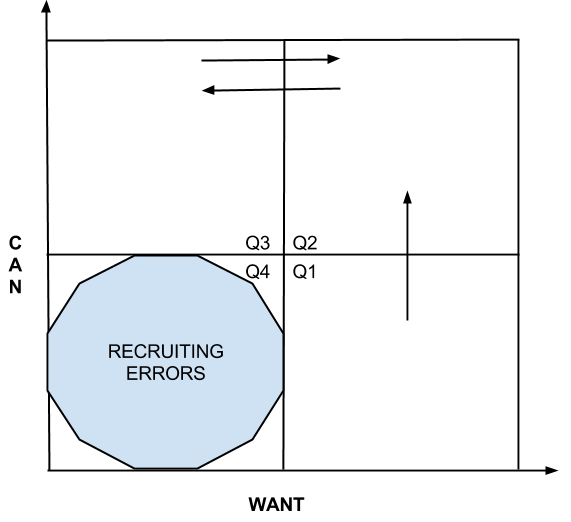
\includegraphics[width=0.8\textwidth]{img/wantcan.png}
\caption{Want-Can Quadrants}
\label{fig:quadrants}
\end{figure}

An employee that usually finds himself in one of the quadrants from \cref{fig:quadrants}. The quadrants are described as:

\begin{description}
\item[Q1] A person wants to do stuff but does not really know how. In this stage are found most of the new employees. The missing knowledge is in most cases represent by the fact the the person does not know the rules and procedures of the company, and it rarely represents the lack of technical information
\item[Q2] Represents employees who want to prove and know the rules of the company and have a drive for adding value to the company. This kind of persons are the most desirable.
\item[Q3] Persons in this stage usually have a few years in the company and have all the necessary knowledge but have lost their desire to work. This de-motivation can come from various cause like: personal problems, company decisions that he does not agree with or routine.
\item[Q4] This are usually recruiting errors, where an employee both has a bad attitude and also a lack of knowledge. The persons in this state are not suitable for the company and they should be terminated as soon as possible, as it will be more costly for the company to develop their skills. On top of that, it may also be impossible because of their unwillingness to work.
\end{description}

The transition from \textit{Q1} to \textit{Q2} is done with little intervention from the manager as long as the company delivers what it promised during the recruiting phase. The slip from \textit{Q2} to \textit{Q3} occurs when the company rules change and the employee does not agree with them or the job is not satisfying enough. In this case the manager has to motivate (financially and professionally) and bring the employee back to \textit{Q2}. Failing to do so will result in the employee leaving the company.
\subsection{PRAE Model}
\label{sub-sec:prae}

Each person has it's own personality and from a psychological point of view there are different indicator types. One of these indicators are the Myers-Brigs indicator \cite{myers} (based on the research of C. Jung) and offer 8 personality traits that result in 16 personality types. This traits are:
\begin{itemize}
\item extroversion(E) / introversion (I)
\item sensing (S) / intuition(N)
\item thinking (T) / feeling (F) 
\item judgement (J) / perception (P)
\end{itemize}
Each person has one of the two traits from each of the categories above, and the different combination result in 16 possible personalities. Their interpretations can be found at \cite{mbf}.

Although the Myers-Brigs indicator was intended to be used by people with no qualifications in psychology, in practice it has proven very difficult for managers to identify the correct traits of their employees without using extensive tests. A simpler model was developed in order to help managers in interacting with their employees based on their personality. 

\begin{figure}[h]
\centering
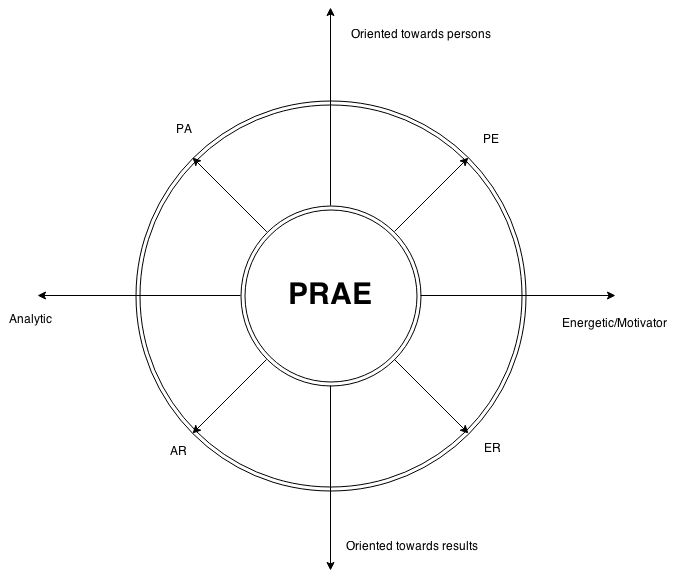
\includegraphics[width=0.8\textwidth]{img/prae.png}
\caption{PRAE personality model}
\label{fig:prae}
\end{figure}

The \textbf{PRAE} model is based on 4 traits, and as the name suggest the traits are:
\begin{itemize}
\item Person oriented
\item Result oriented
\item Analytical
\item Energetic(motivator)
\end{itemize}

Based on the PRAE model, each parson has a dominant trait that he uses in most situations and is usually the way that a person feels most comfortable to act as. A person also has a secondary trait that he usually uses in unusual/under-pressure situations. At the opposite end there is the adverse trait that hints the behaviour that a person is least comfortable to use.

In \ref{fig:prae} the vertical axis (P-R) is called \textit{Scope of action} and the horizontal axis (A-E) is called the \textit{Style of action}. As \ref{fig:prae} hints(although not impossible) the dominant and secondary traits are usually found on different axis. 

Although there are a lot of questionnaires to determine the PRAE model for each person, the dominant and secondary trait can be easily determined by the language that a person uses. In \ref{table:prae} can be found a description of the strong points, weak points and language indicator according to each PRAE trait.

\begin{table}[h]
  \centering
  \caption{Prae dreakdown detalis}
  \setlength\tabcolsep{3.8pt}
  \setlength\extrarowheight{1pt}
    \begin{tabular}{ | p{0.11\textwidth} | p{0.3\textwidth} | p{0.3\textwidth} | p{0.29\textwidth} |}
    \hline
    Trait & Strong points & Week Points & Language Indicators \\ \hline
    
    Person oriented 
     &
      \begin{itemize}
      \item he cares
      \item tactful
      \item motivating
      \item peacemaker, pacifist
      \item looks for cooperation and consensus
      \item tries to involve all the parties
      \end{itemize}
     & 
      \begin{itemize}
      \item easily offend
      \item very emotive
      \item listens to "what the others say"
      \item constantly looking for approval
      \item wishes to please everybody
      \item procrastination in making decisions
      \end{itemize}
     & 
      \begin{itemize}
      \item words like \textit{we, together}
      \item protective vocabulary
      \item do not get straight to the point
      \item spoiled behaviour
      \end{itemize}
     \\ \hline
    Results oriented
     &
      \begin{itemize}
       \item focuses on end result
       \item competitive
       \item honest and straight forward
       \item risk takers
       \item work well under pressure
      \end{itemize}
     &
      \begin{itemize}
       \item do not have patience with people
       \item sometimes sarcastic and insensible
       \item anti rules or processes
       \item individualists
       \item think in black or white
       \item become frustrated by persons who are afraid of risks
      \end{itemize}
     & 
     \begin{itemize}
      \item phrases like: I want
      \item Asks for facts and numbers
      \item Asks \textit {What's in it for me}
      \item Short time spent talking about \textit {how to do it}
     \end{itemize}
     \\ \hline
    Analytical
     &
      \begin{itemize}
       \item precise
       \item looks for proof and validation
       \item plans everything in a step by step way
       \item focused on facts and numbers
       \item sets high standards
      \end{itemize}
     &
      \begin{itemize}
       \item favours processes over results or relationships
       \item tendency to pessimism
       \item critic
       \item suffers from \textit{Paralysis by Analysis}
       \item can portrait intellectual arrogance.
      \end{itemize}
     &
      \begin{itemize}
       \item words like: must and depends
       \item asks for all the details
       \item gets irritated if interrupted
       \item gets frustrated when told how to do his work
      \end{itemize}
     \\ \hline
    Energetic 
     &
      \begin{itemize}
       \item enthusiast
       \item likes variety
       \item creates a friendly environment
       \item persuasive 
       \item spontaneous
       \item likes to have fun
       \item optimist
      \end{itemize}
     &
     \begin{itemize}
      \item impulsive
      \item thinks out loud
      \item disorganized, superficial
      \item easily bored
      \item skips analysis
      \item looks for attention and recognition
     \end{itemize}
     & 
      \begin{itemize}
       \item excessive use of words hinting his person: Me, I 
       \item makes himself the center of attention
       \item reacts positively to phrases like: You can, You will
      \end{itemize}
     \\ \hline
    \end{tabular}
    \label{table:prae}
\end{table}
\FloatBarrier

In the IT industry I observed that in 50\% of cases the combination between dominant and secondary trait is formed from \textit{Analytical} and \textit{Results}. This kind of persons are real assets to a company that is already established and focusses more on quality and not on delivering new features using short deadlines. For continuing to add new value to a product a person that has a mix made from \textit{Results} and \textit{Energetic} person is needed. The biggest drawback I observed for this mix is that this kind of person easily looses it's focus if something new needs to be implement, thus starting to work on new things without analysing all the possible use-cases and delivering software that works only on positive scenarios.
\subsection{RACI Matrix}
\label{sub-sec:raci}
Although not used on large scale in people management a responsibility assignment matrix can be used to help managers in guiding their employees in completing their objectives.
RACI stands for:
\begin{description}
\item[Responsible] The person performing the task. In this case the employee having to complete an objective
\item[Assist] A person that may help the responsible one in completing the task. It may be the manager or a third person with interest in finishing the said objective.
\item[Consulted] A person that may help the responsible person in finishing his task. It usually is a person who already has some experience in the field.
\item[Informed] The person to be update with the status or progress of the objective. This person is usually the manager who sets this objective.
\end{description}
An example of a RACI model can be seen in \cref{table:raciex}
\begin{table}[h]
  \centering
  \caption{RACI example}
  \setlength\tabcolsep{3.8pt}
  \setlength\extrarowheight{1pt}
    \begin{tabular}{ | l | l | l | l | p{3cm} |}
    \hline
    - & Employee & Manager & Team leader & Senior Colleague \\ \hline
    Objective 1 & R & I & - & C \\ \hline
    Objective 2 & R & - & I & C \\ \hline
    Objective 3 & R & I & C & A \\ \hline
    \end{tabular}
    \label{table:raciex}
\end{table}

While I was a people manager, this matrix has proven to be very useful because we would decide in advance who and what would handle, and it always proved to be a point of reference during the objectives following stage, providing the set agreements, thus avoiding excuses like "I though that someone else would have to do this".
\subsection{FAC Model}
\label{sub-sec:fac}
Feedback period is usually a delicate time, it rarely happens when an employee receives only positive feedback. During the evaluation period, a manager has to deliver his view on the employee performance and also the opinions of the colleagues of the evaluated person. 

Seeing that a person will have to receive, sometimes manager apply a technique called \textit{feedback sandwiching} \cite{fbs}. The idea behind this technique is to give merge the positive and negative feedback in such a way that the employee receive good feedback, followed by corrective feedback and so on until it is finished. But this technique may take the employee on an emotional roller-coaster during feedback delivery, confusing him on what he has to do from now on. This combined with the fact that evaluations are done once every 6-12 months the delivery of the feedback may already be too late to correct.

A better solution would be to give constant feedback, as soon as the employees actions require it, in a constructive manner without attacking the persons values while bringing in front the actions that need to be corrected. To do the \textbf{F}acts - \textbf{A}ctions - \textbf{C}orrections can be used. The \textit{FAC} model represents the fact that the context for the actions is put in place, the employee knowing from the start on what situations he is receiving feedback, what he did, what was the outcome and expectations, what he should have done and what are the corrections to be made.

Eg:
`` On Monday evening \textit{(context)}, you have committed the code without compiling the application and causing the build plans to fail, thus blocking the deployment \textit{(facts and outcome)}, while we were expecting you to deploy the new version \textit{(desired actions)}, so the next time please double check that you code does not break the build. ''

This ensures that the employee clearly understands what he did and what, was expected of him without generalizing and also hinting that his specific actions are taken into account, instead of his general way of working.


As a manager tools are a good thing to have, so while starting a process with an employee, a RACI matrix can be developed, while taking into account his PRAE profile to help determine the way to interact and give periodic and constructive feedback can provide useful help in acquiring the end goal.